\documentclass[11pt, a4paper]{article}

\usepackage[top=1 in, bottom = 1 in, left = 1 in, right = 1 in ]{geometry}

\usepackage{amsmath, amssymb, amsfonts}
\usepackage{enumerate}
\usepackage{amsthm}
%\usepackage{pgfplots}
\usepackage{graphicx}

\usepackage[dvipsnames]{xcolor}  


\title{B. Stat - B. Math UGA 2012}
\author{Ananda Biswas}
\date{}

\begin{document}

\maketitle

\begin{enumerate}

	\item[3.]Consider the functions $ f_1 (x) = x $, $ f_2 (x) = 2 + \log_e x $, $ x > 0 $ (where $ e $ is the base of natural logarithm). The graphs of the functions intersect
	\begin{enumerate}[(A)]
		\item once in $ (0,1) $ and never in $ (1, \infty)$
		\item once in $ (0,1) $ and once in $ (e^2, \infty)$
		\item once in $ (0,1) $ and once in $ (e, e^2)$
		\item more than twice in $ (0, \infty)$.
	\end{enumerate}
	
	\begin{flushleft}
	\textbf{Answer ::}
	\end{flushleft}
	
	For $ x = e^{-2} < 1 $, $ f_1 (e^{-2}) = e^{-2}$ and $ f_2 (e^{-2}) = 2 - 2 = 0 $. $ \therefore f_1(e^{-2}) > f_2(e^{-2}) $. $ \ldots \ldots (i) $
	
	Agian for $ x = 1 $, $ f_1 (1) = 1 $ and $ f_2 (1) = 2 $. $ \therefore f_1 (1) < f_2 (1) $. $ \ldots \ldots (ii) $
	
	As $ f_1 $ and $ f_2 $ are always continuous $ \forall x > 0 $, from $ (i) $ and $ (ii) $ we can conclude that, $ f_1 $ and $ f_2 $ must intersect once in $ (e^{-2},1) $. $ 0<e^{-2}<1 $. $ \therefore f_1 $ and $ f_2 $ intersect once in $ (0,1) $.
	
	Again, $ f_1 (e) = e $ and $ f_2 (e) = 2+1 = 3 $. $ 2<e<3 $. $ \therefore f_1(e) < f_2(e) $. $ \ldots \ldots (iii) $
	
	Also, $ f_1 (e^{2}) = e^{2} $ and $ f_2 (e^{2}) = 2+2 = 4 $. $ 4 < e^2 < 9 $. $ \therefore f_1(e^2) > f_2(e^2) $. $ \ldots \ldots (iv) $
	
	From $ (iii) $ and $ (iv) $ we can conclude that, $ f_1 $ and $ f_2 $ must intersect once in $ (e, e^{2}) $. 
	
	\begin{figure}[h]
	\centering
	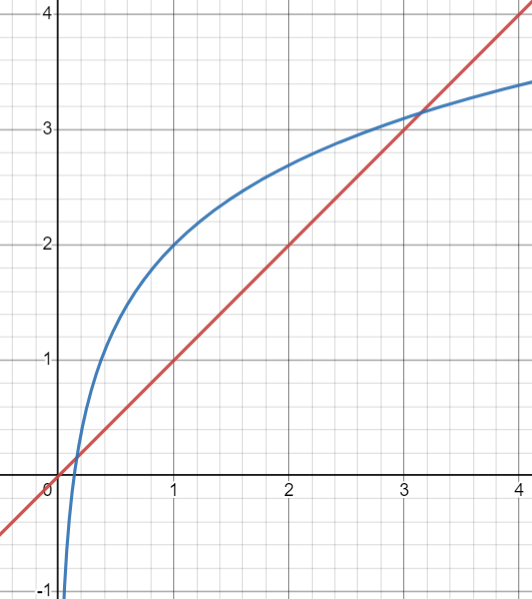
\includegraphics[scale = 0.5]{Screenshot (191)}\\
	\end{figure}
	
	
	\begin{flushright}
	\textbf{(C) once in $ (0,1) $ and once in $ (e, e^2)$ }
	\end{flushright}

	\item[7.] A function $ f : \mathbb{R} \to \mathbb{R} $ is defined by
	\begin{equation*}
	 f(x) =
		\begin{cases}
		 e^{-\frac{1}{x}}, & x > 0  \\
		 0, & x \leq 0.
		\end{cases}
	\end{equation*}
	Then 
	\begin{enumerate}[(A)]
		\item $f$ is not continuous
		\item $f$ is differentiable but $f'$ is not continuous
		\item $f$ is continuous but $f'(0)$ does not exist
		\item $f$ is differentiable and $f'$ is continuous.
	\end{enumerate}
	\begin{flushleft}
	\textbf{Answer ::}
	\end{flushleft}
	From the given information, $f(x)$ is continuous everywhere, except at $x = 0$ where the continuity is questionable. So let's check the continuity of $f(x)$ at $x = 0$. 	
	
	We have $f(0) = 0$;  $ \lim\limits_{x \to 0^{-}} f(x) = 0 $. Now, $\lim\limits_{x \to 0^{+}} f(x) = \lim\limits_{x \to 0} e^{-\frac{1}{x}} = e^{-\infty} = 0 $ \\
	
	$ \therefore \lim\limits_{x \to 0^{-}} f(x) = f(0) = \lim\limits_{x \to 0^{+}} f(x)  $  $ \therefore f(x)$ is continuous at $ x = 0 $ and hence $f(x)$ is continuous everywhere.
	
	Again from the given information, $f(x)$ is differentiable everywhere, except at $x = 0$ where the differentiability is questionable. So now let's check the differentiability of $f(x)$ at $x = 0$.
	
	Now, $\lim\limits_{x \to 0^{-}} \dfrac{f(x) - f(0)}{x - 0} = \lim\limits_{x \to 0} \dfrac{0}{x} = 0 $.
	
	And, $ \lim\limits_{x \to 0^{+}} \dfrac{f(x) - f(0)}{x - 0} = \lim\limits_{x \to 0} \dfrac{e^{-\frac{1}{x}}}{x} = \lim\limits_{h \to \infty} he^{-h} = \lim\limits_{h \to \infty} \dfrac{h}{e^h} = \dfrac{\text{tends to}\, \infty}{\text{tends to}\, e^{\infty}} = 0 $. \Big[ $x = \dfrac{1}{h}$ \Big]
	
	$ \therefore $ $Lf'(0) = Rf'(0)$. $ \therefore f(x)$ is differentiable at $ x = 0 $ and hence $f(x)$ is differentiable everywhere.
	
	Now, \begin{equation*}
	 f'(x) =
		\begin{cases}
		 \dfrac{e^{-\frac{1}{x}}}{x^2} , & x > 0 \\
		 
		 0, & x \leq 0.
		\end{cases}
	\end{equation*}
	
	Clearly, $f'(0) = 0$;  $ \lim\limits_{x \to 0^{-}} f'(x) = 0 $. 
	
	Now, $\lim\limits_{x \to 0^{+}} f'(x) = \lim\limits_{x \to 0} \dfrac{e^{-\frac{1}{x}}}{x^2} = \lim\limits_{h \to \infty} h^2e^{-h} = \lim\limits_{h \to \infty} \dfrac{h^2}{e^h} = \dfrac{\text{tends to}\, \infty}{\text{tends to}\, e^{\infty}} = 0 $ \\
	
	So, $f'$ is continuous everywhere.
	
	\begin{flushright}
	\textbf{(D) $f$ is differentiable and $f'$ is continuous.}
	\end{flushright}
	
	\item[19.]What is the limit of 
	$$ \left( 1 + \dfrac{1}{n^2 + n} \right)^{n^2 + \sqrt{n}} $$
	
	as $ n \to \infty $?
	\begin{enumerate}[(A)]
	\item $ e $
	\item $ 1 $
	\item $ 0 $
	\item $ \infty $.
	\end{enumerate}
	
	\begin{flushleft}
	\textbf{Answer ::}
	\end{flushleft}
	
	The given limit is of the format $ 1^{\infty} $.
	
	So, the result of the limit is of the form $ e^A $ where $ A = \lim\limits_{n \to \infty} \left( \dfrac{n^2 + \sqrt{n}}{n^2 + n} \right)$.
	
	Now, $ A = \lim\limits_{n \to \infty} \left( \dfrac{1 + \frac{1}{n\sqrt{n}} }{1 + \frac{1}{n}} \right)  = \left( \dfrac{1+0}{1+0}  \right) = 1 $.
	
	$ \therefore \lim\limits_{n \to \infty} \left( 1 + \dfrac{1}{n^2 + n} \right)^{n^2 + \sqrt{n}} = e^1 = e $.
	
	\begin{flushright}
	\textbf{(A) $e$}
	\end{flushright}

	\item[20.] 
	Consider the function $ f(x) = x^4 + x^2 + x -1 $, $ x \in (-\infty,\infty) $. The function
		\begin{enumerate}[(A)]
	 	\item is zero at $ x = -1 $, but is increasing near $ x = -1 $
	 	\item has a zero in  $(-\infty, -1)$
	 	\item has two zeros in $ (-1, 0) $
	 	\item has exactly one local minimum in $ (-1, 0) $.
		\end{enumerate}
	
	\begin{flushleft}
	\textbf{Answer ::}
	\end{flushleft}
	$ f(-1) = 1+1-1-1 = 0 $, $ f(0) = 0+0+0-1 = -1 $ and $ f(1) = 1+1+1-1 = 2 $
	
	So there is a root of $ f(x) $ in (0,1).
	
	$ f(x) $ is a polynomial. So $ f(x) $ is continuous and differentiable everywhere. $ f(x) $ is concave up and its graph looks like this.
	\begin{figure}[h]
	\centering
	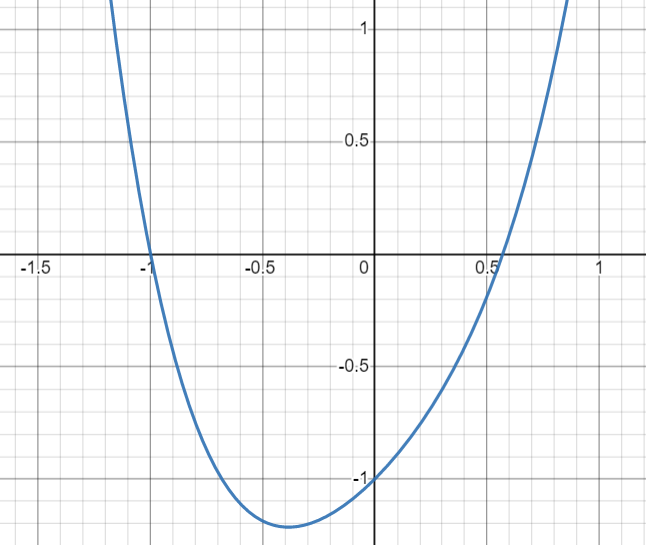
\includegraphics[scale = 0.5]{Screenshot (181)}\\
	\end{figure}

	Clearly, $ \forall x \in (-\infty, -1) $, $ f(x) > 0 $.
	
	So, option (B) is incorrect.
	
	$ \therefore $ $ f'(x) = 4x^3 + 2x + 1 $. $ \therefore $ $ f'(-1) = -4 - 2 + 1 = -5 < 0 $. So $f(x)$ is decreasing at $ x = -1 $
	
	So, option (A) is incorrect.
	
	Again, $ f'(1) = 4+2+1 = 7 > 0 $. So $f(x)$ is increasing at $ x = 1 $
	
	Also, $ f'(0) = 0+0+1 = 1 > 0 $. So $f(x)$ is increasing at $ x = 0 $
	
	Observe that, $ f'(-1) < 0 $ and $ f'(0) > 0 $. So $ \exists c \in (-1,0) $ such that, $ f'(c) = 0 $. And at $ c $, the change of sign must be from negative to positive.
	
	So, $ f(x) $ has one local minimum in $ (-1,0) $. Now we have to check whether this is the only minimum in $ (-1,0) $.
	
	Now, $ f''(x) = 12x^2 + 2 $. So, $ f''(x) > 0 $ $\forall x \in (-1,0) $. So, $ f'(x) $ is always increasing in $ (-1,0) $. Therefore, $f'(x)$ can have maximum one root in between $ (-1,0) $. So, there exists only one $ c \in  (-1,0) $ such that $ f'(c) = 0 $. Hence, $ f(x) $ has exactly one local minimum in $ (-1,0) $.
	
	So, option (D) is correct.
	
	We shall also show that, $ f(x) $ cannot have two zeros in $ (-1,0) $. If so, then the graph of $ f(x) $ must look like this.\\
	\begin{figure}[h]
	\centering
	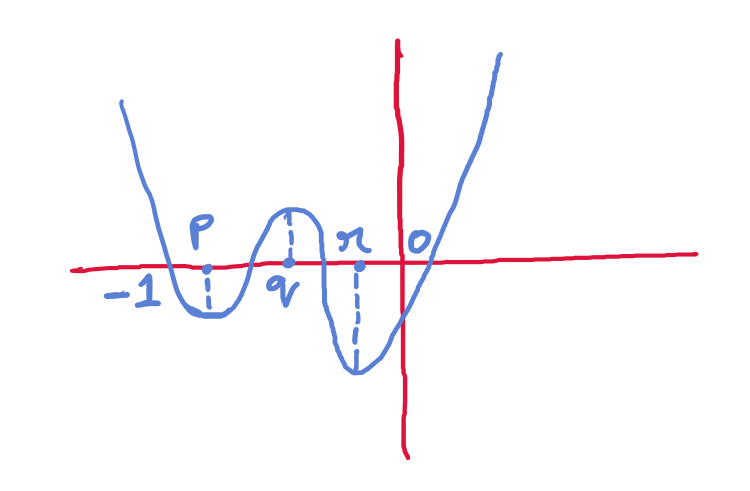
\includegraphics[scale = 0.5]{Screenshot (182)}\\
	\end{figure}
	\pagebreak

	Then we would have 3 points $p$, $q$, $r$ such that $f'$ is zero. But we just showed that in $ (-1,0) $, $f'$ cannot have more than one root. Consequently, in $ (-1,0) $, $ f $ cannot have any zero.
	\begin{flushright}
	\textbf{(D) has exactly one local minimum in $ (-1,0) $}
	\end{flushright}

\end{enumerate}



\end{document}